% UN PO DI IMPORT
\documentclass{article}
\usepackage[utf8]{inputenc}
\usepackage{graphicx}
\graphicspath{ {./images/} }
\usepackage[svgnames]{xcolor}
\usepackage{listings}
\usepackage{xcolor} % Per il colore del testo
\usepackage{fontawesome5}


% Definizione del nuovo comando
\newcommand{\tabb}[1]{\texttt{\textcolor{blue}{#1}}}
\newcommand{\tab}[1]{\texttt{\textcolor{cyan}{#1}}}
\newcommand{\attr}[1]{\texttt{\textcolor{gray}{#1}}}
\newcommand{\sqlcommand}[1]{\texttt{\textcolor{orange}{#1}}}
\newcommand{\sqlfunc}[1]{\texttt{\textcolor{violet}{#1}}}
\newcommand{\sqltrigger}[1]{\texttt{\textcolor{teal}{#1}}}
\newcommand{\sqlview}[1]{\texttt{\textcolor{yellow}{#1}}}
\newcommand{\m}[1]{\texttt{}}
\newcommand{\und}[0]{\textunderscore}
\newcommand{\alert}[0]{\textcolor{red}{\faExclamationCircle}}
\newcommand{\danger}[0]{\textcolor{red}{\faExclamationCircle}}


\title{PiGEU\\ Piattaforma per la Gestione degli Esami Universitari}
%\subtitle{DOCUMENTAZIONE TECNICA}

\author{\textbf{DOCUMENTAZIONE TECNICA}}
\date{Fontana Francesco \\ matr. 943519}

\begin{document}

    \maketitle

    \begin{abstract}

        La Piattaforma per la Gestione degli Esami Universitari, d'ora in poi chiamata PiGEU per comodità, è una soluzione che permette di gestire
        uno scenario universitario in cui siano presenti insegnamenti e corsi di laurea, docenti, studenti e segretari, iscrizioni e verbalizzazioni
        ai diversi appelli di esame di ogni insegnamento, generazione di documentazioni valide per gli studenti quali i certificati di carriera, visibili
        o anche scaricabili in formato PDF.

        PiGEU, nel suo complesso, abbraccia principalmente quattro tecnologie, quali:
        \begin{itemize}
            \item \textbf{PostgreSQL} per la gestione del database nel quale tramite \emph{tabelle} vi è la memorizzazione dei dati di tutte
            le entità coinvolte, tramite \emph{trigger} vengono controllate alcune proprietà della base di dati per preservare la consistenza dell'informazione e rispettare le specifiche fornite
            \item \textbf{HTML} come linguaggio di markup per rendere l'accesso ai dati maggiormente fruibile e comprensibile da parte dell'utente, rappresentando i dati in forma testuale o grafica (tabelle) e consentendo la possibilità di interrogare la base di dati mediante bottoni. Questo linguaggio è usato per rendere PiGEU maggiormente \emph{user-friendly}
            \item \textbf{PHP} linguaggio di scripting server-side che "abbraccia" le due tecnologie sopra indicate, utilizzato per:
            \begin{itemize}
                \item eseguire in linguaggio SQL-DML le interrogazioni al database che vengono fatte da parte dell'utente tramite la compilazione di form in HTML, inviate tramite la pressione di bottoni HTML
                \item realizzare documenti in PDF tramite l'apposita libreria TCPDF
            \end{itemize}
            \item \textbf{Javascript}, linguaggio di scripting (usato in questo caso per la parte client-side) che è stato utilizzato per
            \begin{itemize}
                \item eseguire chiamate AJAX migliorando la performance di navigazione
                \item eseguire interrogazioni al database in maniera più semplice, senza la pressione di bottoni di submit ma solamente con la digitazione da tastiera ad esempio durante la ricerca di una utenza
            \end{itemize}
        \end{itemize}
        L'intero sviluppo del progetto in tutte le sue fasi, è documentato in un apposito repository di Github al seguente link \url{https://github.com/ffont28/PiGEU } di cui qui sotto viene mostrata un'immagine indicante gli stati di commit
        \includegraphics[scale=0.437]{images/PiGEU-history.png}
    \end{abstract}

    \pagebreak

    \tableofcontents

    \pagebreak

    \section{Schema concettuale (ER) della base di dati}
    Di seguito lo schema concettuale alla base della progettazione della base di dati.
    Lo schema seguente è stato successivamente ristrutturato per la realizzazione dello schema logico, dato che la relazione in linguaggio SQL-DDL viene espressa con una tabella.


    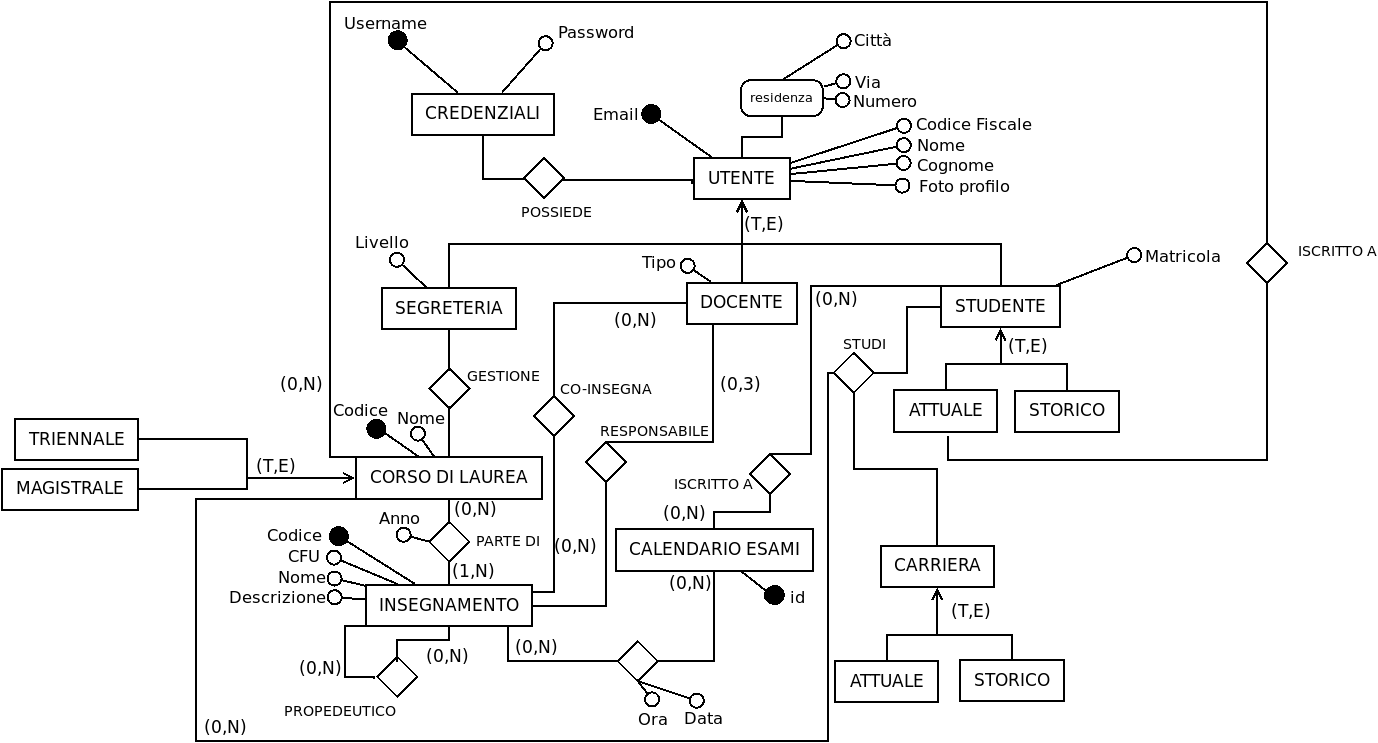
\includegraphics[scale=0.25]{images/SchemaER_PiGEU.png}

    \section{Schema logico (relazionale) della base di dati}
    Di seguito viene fornito lo schema logico della base di dati di PiGEU, tramite i comandi DDL utilizzati. La base di dati contiene 19 tabelle: per ognuna di esse verrà eventualmente fornito qualche commento per spiegare al meglio le scelte implementative derivanti dalle specifiche assegnate

    \lstset{
        basicstyle=\footnotesize,
        keywordstyle=\color{MidnightBlue}\bfseries,
        identifierstyle=\color{Purple},
        commentstyle=\color{Green}\itshape,
        stringstyle=\color{Red}\ttfamily,
        showstringspaces=false,
        numbers=left, numberstyle=\tiny,
        stepnumber=1, numbersep=5pt,
        tabsize=4,
        framexleftmargin=5mm, rulesepcolor=\color{LightGray},
        frame=LtBr,
        language={SQL}, ##
        mathescape=true,
        fontadjust=true,
        breaklines=true,breakatwhitespace=true,breakautoindent
    }

    \begin{enumerate}
        \item La tabella \tabb{utente} contiene i dati di qualsiasi utente, che sia di tipo \emph{segreteria}, \emph{studente} oppure \emph{docente}. Questa soluzione di utenza generica è pensata appositamente nell'ottica della \emph{scalabilità} di questo software, così da poter aggiungere anche altri tipi di utenze mediante ulteriori tabelle.

        Questa tabella contiene i dati fondamentali di un utente, quali l'\texttt{email} che è l'identificatore univoco (chiave primaria) di ciascun utente nel database, corrisponde a quella che è l'email istituzionale di università, il suo \texttt{nome} e \texttt{cognome}, il suo \texttt{indirizzo} e \texttt{città} di residenza, il suo \texttt{codice fiscale} da cui si può desumere \textbf{la data di nascita} e il \textit{luogo di nascita} e da ultimo l'\texttt{emailpersonale} che rappresenta la mail di recupero dell'utente, al di fuori del dominio email di università.
        \begin{lstlisting}[
            language={SQL},
            title={Utente}]
CREATE TABLE public.utente (
    email character varying(50) NOT NULL,
    nome character varying(50),
    cognome character varying(50),
    indirizzo character varying(255),
    citta character varying(255),
    codicefiscale character varying(16),
    emailpersonale character varying(60),
    PRIMARY KEY (email)
);
        \end{lstlisting}

        \item La tabella \tabb{credenziali} contiene per ciascun utente (denominato \attr{username}), la corrispettiva \attr{password} cifrata con l'algoritmo MD5. Il senso di questa tabella è, come è facile intuire, poter garantire l'accesso solamente agli utenti autorizzati.
        \begin{lstlisting}[
            language={SQL},
            title={credenziali}]
CREATE TABLE public.credenziali (
    username character varying(50) NOT NULL,
    password character varying(50),
    PRIMARY KEY (username),
    FOREIGN KEY (username) REFERENCES public.utente(email) ON UPDATE CASCADE ON DELETE CASCADE
);
        \end{lstlisting}

        \item La tabella \tabb{Segreteria} contiene i dati degli utenti di tipo \textit{segreteria} identificati da un livello come ad esempio la segreteria del personale piuttosto che la segreteria studenti o segreteria didattica. L'attributo \texttt{utente} referenzia l'\attr{email} della tabella \tab{Utente}
        \begin{lstlisting}[
            language={SQL},
            title={Segreteria}]
CREATE TABLE public.segreteria (
    utente character varying(50) NOT NULL,
    livello character varying(9) NOT NULL,
    PRIMARY KEY (utente),
    FOREIGN KEY (utente) REFERENCES public.utente(email) ON UPDATE CASCADE ON DELETE CASCADE
);
        \end{lstlisting}

        \item La tabella \tabb{Docente} contiene i dati degli utenti di tipo \textit{docente}. Oltre a referenziare l'\attr{email} della tabella \tab{Utente}, contiene anche un attributo \attr{tipo} che indica il tipo di docente, ad esempio "ordinario", "associato", "a contratto",...
        \begin{lstlisting}[
            language={SQL},
            title={Docente}]
CREATE TABLE public.docente (
    utente character varying(50) NOT NULL,
    tipo character varying(50),
    PRIMARY KEY (utente),
    FOREIGN KEY (utente) REFERENCES public.utente(email) ON UPDATE CASCADE ON DELETE CASCADE
);
        \end{lstlisting}

        \item La tabella \tabb{Studente} contiene i dati degli utenti di tipo \textit{studente}. Anch'essa referenzia l'\attr{email} della tabella \tab{Utente}, e contiene due attributi caratteristici di uno stuente:
        \begin{itemize}
            \item l'attributo \attr{matricola} che indica la matricola dello studente
            \item l'attributo \attr{corso\und di\und laurea} in riferimento al corso di laurea a cui risulta iscritto lo studdente
        \end{itemize}
        \begin{lstlisting}[
            language={SQL},
            title={Studente}]
CREATE TABLE public.studente (
    utente character varying(50) NOT NULL,
    matricola serial NOT NULL,
    corso_di_laurea character varying(5),
    PRIMARY KEY (utente),
    FOREIGN KEY (corso_di_laurea) REFERENCES public.corso_di_laurea(codice) ON UPDATE CASCADE ON DELETE CASCADE,
    FOREIGN KEY (utente) REFERENCES public.utente(email) ON UPDATE CASCADE ON DELETE CASCADE
);
        \end{lstlisting}

        \item La tabella \tabb{Corso\und di\und laurea} contiene i dati di un corso di laurea, quali:
        \begin{itemize}
            \item il \attr{codice}, identificatore univoco di uno specifico corso di laurea
            \item il \attr{nome} del corso di laurea
            \item il \attr{tipo} del corso di laurea, che può essere
            \begin{itemize}
                \item \textit{triennale}, ovvero della durata di tre anni
                \item \textit{magistrale} ovvero della durata di due anni
                \item \textit{magistrale a ciclo unico} della durata di cinque anni
            \end{itemize}
        \end{itemize}
        \begin{lstlisting}[
            language={SQL},
            title={Corso di Laurea}]
CREATE TABLE public.corso_di_laurea (
    codice character varying(5) NOT NULL,
    nome character varying(50),
    tipo character varying(50),
    PRIMARY KEY (codice)
);
        \end{lstlisting}

        \item La tabella \tabb{Insegnamento} contiene i dati relativi a un insegnamento, quali:
        \begin{itemize}
            \item il \attr{codice}, identificatore univoco di uno specifico insegnamento
            \item il \attr{nome} dell'insegnamento
            \item una \attr{descrizione} testuale dell'insegnamento, che enumera le conoscenze che tale disciplina vuole trasmettere allo studente
            \item i \attr{cfu}, ovvero i crediti formativi universitari che l'insegnamento attribuisce allo studente che consegue un profitto in questa disciplina
        \end{itemize}
        \alert l'attributo indicante l'\textit{anno} in cui è previsto l'insegnamento è volutamente omesso e verrà specificata la motivazione succesivamente nella descrizione della tabella \tab{insegnamento\und parte\und di\und cdl}
        \begin{lstlisting}[
            language={SQL},
            title={Insegnamento}]
CREATE TABLE public.insegnamento (
    codice character varying(10) NOT NULL,
    nome character varying(50),
    descrizione text,
    cfu character(2),
    PRIMARY KEY (codice)
);
        \end{lstlisting}

        \item Ogni insegnamento ha un \tabb{docente\und responsabile} ovvero un docente che si occupa dell'organizzazione didattica dell'insegnamento come ad esempio, come vedremo in seguito, la pianificazione del calendario esami per l'insegnamento, e la verbalizzazione degli esiti degli esami dell'insegnamento.
        Questa tabella quindi indica la relazione tra un \attr{docente} e un \attr{insegnamento} i quali referenziano le omonime tabelle nelle loro chiavi primarie.
        \begin{lstlisting}[
            language={SQL},
            title={Docente Responsabile}]
CREATE TABLE public.docente_responsabile (
    docente character varying(50) NOT NULL,
    insegnamento character varying(10) NOT NULL
    PRIMARY KEY (docente, insegnamento),
    FOREIGN KEY (docente) REFERENCES public.docente(utente) ON UPDATE CASCADE ON DELETE CASCADE,
    FOREIGN KEY (insegnamento) REFERENCES public.insegnamento(codice) ON UPDATE CASCADE ON DELETE CASCADE
);
        \end{lstlisting}

        \item Ogni insegnamento può avere uno o più docenti: la tabella \tabb{insegnamento} esprime questa relazione. Questa tabella conterrà solamente i docenti di un insegnamento che non siano già responsabili di quell'insegnamento. Come nella tabella \tab{docente\und responsabile} i due attributi fanno riferimento a un docente e a un insegnamento.
        \begin{lstlisting}[
            language={SQL},
            title={Insegna}]
CREATE TABLE public.insegna (
    docente character varying(50) NOT NULL,
    insegnamento character varying(10) NOT NULL,
    PRIMARY KEY (docente, insegnamento),
    FOREIGN KEY (docente) REFERENCES public.docente(utente) ON UPDATE CASCADE ON DELETE CASCADE,
    FOREIGN KEY (insegnamento) REFERENCES public.insegnamento(codice) ON UPDATE CASCADE ON DELETE CASCADE
);
        \end{lstlisting}

        \item La tabella \tabb{insegnamento\und parte\und di\und cdl} descrive la relazione per la quale ogni insegnamento non sia a se stante, ma faccia parte di un determinato corso di laurea.


        \alert Si noti che una scelta implementativa che diverge dalle specifiche è inserire l'attirbuto \attr{anno} all'interno di questa relazione e non come proprietà di un singolo corso di laurea, dal momento che uno stesso insegnamento può essere erogato in più corsi di laurea in anni diversi (ad esempio l'insegnamento \texttt{i} può essere erogato per il corso di laurea \texttt{c1} al primo anno, mentre per il corso di laurea \texttt{c2} al terzo anno)

        \begin{lstlisting}[
            language={SQL},
            title={Insegnamento parte di un Corso di Laurea}]
CREATE TABLE public.insegnamento_parte_di_cdl (
    insegnamento character varying(10) NOT NULL,
    corso_di_laurea character varying(5) NOT NULL,
    anno integer NOT NULL,
    PRIMARY KEY (insegnamento, corso_di_laurea, anno),
    FOREIGN KEY (corso_di_laurea) REFERENCES public.corso_di_laurea(codice) ON UPDATE CASCADE ON DELETE CASCADE,
    FOREIGN KEY (insegnamento) REFERENCES public.insegnamento(codice) ON UPDATE CASCADE ON DELETE CASCADE
);
        \end{lstlisting}

        \item La tabella \tabb{propedeuticita} descrive la relazione per la quale eventualmente un insegnamento \attr{insegnamento1} possa essere propedeutico a un altro insegnamento \attr{insegnamento2} all'interno di un \attr{corso\und di\und laurea}. Anche qui è importante notare come un insegnamento sia propedeutico a un altro solamente nel contesto di un corso di laurea, non in maniera assoluta.

        \begin{lstlisting}[
            language={SQL},
            title={Propedeuticità}]
CREATE TABLE public.propedeuticita (
    insegnamento1 character varying(10) NOT NULL,
    insegnamento2 character varying(10) NOT NULL,
    corso_di_laurea character varying(5) NOT NULL,
    PRIMARY KEY (insegnamento1, insegnamento2, corso_di_laurea),
    FOREIGN KEY (insegnamento1) REFERENCES public.insegnamento(codice) ON UPDATE CASCADE ON DELETE CASCADE,
    FOREIGN KEY (insegnamento2) REFERENCES public.insegnamento(codice) ON UPDATE CASCADE ON DELETE CASCADE
    FOREIGN KEY (corso_di_laurea) REFERENCES public.corso_di_laurea(codice) ON UPDATE CASCADE ON DELETE CASCADE
);
        \end{lstlisting}

        \item La tabella \tabb{insegnamenti\und per\und carriera} esprime un sottile concetto presente nell'ambito universitario: all'atto dell'immatricolazione a uno studente viene attribuito un \textit{piano di studi} che è rappresentato proprio da questa tabella: a ogni studente viene assegnato un elenco di insegnamenti da superare. Se successivamente all'immatricolazione dello studente (che qui coincide con l'atto dell'inserimento nel database) in un dato corso di laurea viene inserito un nuovo insegnamento, non viene modificato il piano di studi dello studente già iscritto precedentemente la modifica. L'attributo \attr{timestamp} serve per tenere una marca temporale dell'atto della realizzazione del presente piano di insegnamenti da superare. Un'ulteriore indicazione di quanto detto finora è dato dal \textbf{vincolo di chiave esterna} che referenzia solamente l'attributo \textbf{utente} della tabella \tab{studente} (e non anche il \textbf{codice} la tabella \tab{insegnamento}!): se lo studente \texttt{s} viene rimosso dalla tabella \tab{studente} ad esempio perchè abbandona gli studi oppure si è laureato (in questo caso i dati verranno spostati in apposite tabelle di \textit{storico} che verranno mostrate in seguito), decade l'insieme di insegnamenti di cui superare gli esami ai fini della carriera. Qualora \texttt{s} volesse reiscriversi, si troverebbe assegnati gli insegnamenti di cui conseguire profitto all'atto della nuova iscrizione.
        \begin{lstlisting}[
            language={SQL},
            title={Insegnamenti per carriera}]
CREATE TABLE public.insegnamenti_per_carriera (
    studente character varying(50) NOT NULL,
    insegnamento character varying(10) NOT NULL,
    "timestamp" timestamp(6) without time zone,
    PRIMARY KEY (studente, insegnamento),
    FOREIGN KEY (studente) REFERENCES public.studente(utente) ON UPDATE CASCADE ON DELETE CASCADE
);
        \end{lstlisting}

        \item La tabella \tabb{calendario\und esami} rappresenta un calendario di esami in cui vengono indicati:
        \begin{itemize}
            \item un \attr{insegnamento} che referenzia l'attributo \textit{codice} della tabella \tabb{insegnamento}
            \item la \attr{data} dell'esame
            \item l' \attr{ora} dell'esame
            \item un \attr{id} univoco identificativo di uno specifico \textit{esame} che è costituito dalla tripla sopra indicata, ovvero $\langle$\textit{insegnamento}, \textit{data}, \textit{ora}$\rangle$

        \end{itemize}
        \begin{lstlisting}[
            language={SQL},
            title={Calendario Esami}]
CREATE TABLE public.calendario_esami (
    insegnamento character varying(10) NOT NULL,
    data date NOT NULL,
    ora time without time zone NOT NULL,
    id serial PRIMARY KEY,
    FOREIGN KEY (insegnamento) REFERENCES public.insegnamento(codice) ON UPDATE CASCADE ON DELETE CASCADE
);
        \end{lstlisting}

        \item La tabella \tabb{iscrizione} esprime l'iscrizione di uno \attr{studente} a un \attr{esame}, quest'ultimo attributo che referenzia la tabella \tab{calendario\und esami} nel suo attributo \attr{id}
        \begin{lstlisting}[
            language={SQL},
            title={Iscrizione}]
CREATE TABLE public.iscrizione (
    studente character varying(50) NOT NULL,
    esame integer NOT NULL,
    PRIMARY KEY (studente, esame),
    FOREIGN KEY (studente) REFERENCES public.studente(utente) ON UPDATE CASCADE ON DELETE CASCADE,
    FOREIGN KEY (esame) REFERENCES public.calendario_esami(id) ON UPDATE CASCADE ON DELETE CASCADE
);
        \end{lstlisting}

        \item La tabella \tabb{Carriera} contiene i dati della carriera di ciascun studente, ovvero per ogni \attr{insegnamento} di cui sia stato sostenuto \textit{almeno} un esame, la corrispettiva \attr{valutazione} conseguita in tal \attr{data}. Si noti l'enfasi sul termine "almeno" per indicare che in carriera vengono registrati tutti i tentativi di sostenimento di esame, essendo stabilita come chiave primaria la tripla $\langle$\textit{studente}, \textit{insegnamento}, \textit{data}$\rangle$ è costituita quella che in gergo viene detta \textit{serie storica}.
        \begin{lstlisting}[
            language={SQL},
            title={Carriera}]
CREATE TABLE public.carriera (
    studente character varying(50) NOT NULL,
    insegnamento character varying(10) NOT NULL,
    valutazione smallint,
    data date NOT NULL,
    PRIMARY KEY (studente, data, insegnamento),
    FOREIGN KEY (studente, insegnamento) REFERENCES public.insegnamenti_per_carriera(studente, insegnamento) ON UPDATE CASCADE ON DELETE CASCADE
);
        \end{lstlisting}

        \item La tabella \tabb{utente\und storico} contiene gli utenti inseriti in storico. Per il momento l'unica tipologia di utenti per cui è previsto lo storico sono gli \textit{studenti}. La struttura e la semantica è del tutto identica alla tabella \tab{utente}
        \begin{lstlisting}[
            language={SQL},
            title={Utente Storico}]
CREATE TABLE public.utente_storico (
    email character varying(50) NOT NULL,
    nome character varying(50),
    cognome character varying(50),
    indirizzo character varying(255),
    citta character varying(255),
    codicefiscale character varying(16),
    emailpersonale character varying(60),
    PRIMARY KEY (email)
);
        \end{lstlisting}

        \item La tabella \tabb{studente\und storico} contiene i dati degli studenti inseriti in storico. La struttura e la semantica è del tutto identica alla tabella \tab{studente}
        \begin{lstlisting}[
            language={SQL},
            title={Studente Storico}]
CREATE TABLE public.studente_storico (
    utente character varying(50) NOT NULL,
    matricola integer,
    corso_di_laurea character varying(5),
    PRIMARY KEY (utente),
    FOREIGN KEY (utente) REFERENCES public.utente_storico(email) ON UPDATE CASCADE ON DELETE CASCADE
);
        \end{lstlisting}

        \item La tabella \tabb{carriera\und storico} contiene i dati della carriera di studenti inseriti in storico. La struttura e la semantica è del tutto identica alla tabella \tab{carriera}
        \begin{lstlisting}[
            language={SQL},
            title={Carriera Storico}]
CREATE TABLE public.carriera_storico (
    studente character varying(50) NOT NULL,
    insegnamento character varying(10) NOT NULL,
    valutazione smallint,
    data date NOT NULL,
    PRIMARY KEY (studente, insegnamento, data),
    FOREIGN KEY (studente) REFERENCES public.studente_storico(utente) ON UPDATE CASCADE ON DELETE CASCADE
);
        \end{lstlisting}

        \item La tabella \tabb{foto\und profilo} contiene, per ciascun \attr{utente}, il corrispettivo percorso interno al server in cui si trova l'immagine del profilo, tramite l'attributo \attr{path}. Inoltre l'attirbuto \attr{timestamp} serve per tenere memoria delle vecchie foto profilo dell'utente in questione.
        \begin{lstlisting}[
            language={SQL},
            title={Foto Profilo}]
CREATE TABLE public.foto_profilo (
    utente character varying(50) NOT NULL,
    path character varying(200),
    "timestamp" timestamp(6) without time zone NOT NULL,
    PRIMARY KEY (utente, "timestamp"),
    FOREIGN KEY (utente) REFERENCES public.utente(email) ON UPDATE CASCADE ON DELETE CASCADE
);
        \end{lstlisting}
    \end{enumerate}

    \section{Esauriente descrizione delle funzioni realizzate}
    \subsection{Funzioni SQL-DML Richieste}
    Questa sezione ha lo scopo di mostrare le funzioni in linguaggio SQL per la manipolazione dei dati interni al lato PostgreSQL di PiGEU. Per ciascuna funzione verrà mostrata l'ulitità ed eventuali osservazioni.
    \subsubsection{Rimozione di uno studente - [specifica 2.2.1]}
    Nelle specifiche indicate, la rimozione di uno studente \texttt{s} non corrisponde con il solo comando di \sqlcommand{DELETE} all'interno della tabella \tabb{utente} ma comporta il trasferimento di tutte le informazioni relative ad \texttt{s} in apposite tabelle di \textit{storico}. La funzione \sqlfunc{sposta\und dati\und studente} contiene diversi comandi DML che consentono di soddisfare le specifiche. Di seguito il codice sorgente della funzione che oltre alle operazioni richieste, restituisce anche un messaggio di stato oppure, nel caso di sollevamento di eccezioni, il messaggio di eccezione.

    \pagebreak
    \begin{lstlisting}[
    language={SQL},
    title={sposta\und dati\und studente(\texttt{E} \attr{varchar})}]
    CREATE OR REPLACE FUNCTION sposta_dati_studente(E varchar) RETURNS TEXT AS $$
    DECLARE
    status TEXT := 'Dati spostati con successo.';
    BEGIN
    -- INSERT utente --> utente_storico
    INSERT INTO utente_storico (email, nome, cognome, indirizzo, citta, codicefiscale, emailpersonale)
    SELECT email, nome, cognome, indirizzo, citta, codicefiscale, emailpersonale
    FROM utente where email = $1;

    -- INSERT studente --> studente_storico
    INSERT INTO studente_storico (utente, matricola, corso_di_laurea)
    SELECT utente, matricola, corso_di_laurea
    FROM studente WHERE utente = $1;

    -- INSERT carriera --> carriera_storico
    INSERT INTO carriera_storico (studente, insegnamento, valutazione, data)
    SELECT studente, insegnamento, valutazione, data
    FROM carriera WHERE studente = $1;

    -- cancello i dati dalla tabella utente dopo averli spostati in utente_storico
    DELETE FROM utente where email = $1;
    -- le seguenti operazioni sono fatte gia' in CASCADE
    -- cancello i dati dalla tabella studente dopo averli spostati in stutente_storico
    -- DELETE FROM studente WHERE utente = $1;
    -- cancello i dati dalla tabella carriera dopo averli spostati in carriera_storico
    -- DELETE FROM carriera WHERE email = $1;
    -- cancello i dati dalla tabella insegnamenti_per_carriera
    -- DELETE FROM insegnamenti_per_carriera WHERE studente = $1;
    RETURN status;
    -- Gestione delle eccezioni
    EXCEPTION
    WHEN OTHERS THEN
    -- In caso di errore restituisco il messaggio di errore
    status := 'Errore: ' || SQLERRM;
    RETURN status;
    END;
    $$ LANGUAGE plpgsql;
\end{lstlisting}
\subsubsection{Correttezza delle iscrizioni agli esami - [specifica 2.2.2]}
Nella \textit{specifica 2.2.2} viene detto che
\begin{quote}
    Ciascuno studente può iscriversi ad un esame solo se l'insegnamento è previsto dal proprio corso di laurea, e solamente se tutte le propedeuticità sono rispettate.
\end{quote}

\begin{itemize}
    \item La prima condizione, cioé la possibilità di iscrizione ai soli esami di insegnamenti del proprio corso di laurea, viene controllata tramite un trigger denominato \sqltrigger{no\und iscriz\und se\und non\und in\und CdL} di cui viene fornito il codice sorgente
    \begin{lstlisting}[
        language={SQL},
        title={\texttt{no\und iscriz\und se\und non\und in\und CdL}}]
CREATE OR REPLACE TRIGGER no_iscriz_se_non_in_CdL
    BEFORE INSERT OR UPDATE ON iscrizione
    FOR EACH ROW
EXECUTE FUNCTION check_appartenenza_cdl();
    \end{lstlisting}
    Tale trigger prima che venga inserita una riga nella tabella \tabb{iscrizione} chiama l'esecuzione della funzione \sqlfunc{check\und appartenenza\und cdl} di seguito mostrata
    \begin{lstlisting}[
        language={SQL},
        title={\texttt{check\und appartenenza\und cdl()}}]
CREATE OR REPLACE FUNCTION check_appartenenza_cdl() RETURNS TRIGGER as $$
BEGIN
    PERFORM * FROM calendario_esami c
            INNER JOIN insegnamenti_per_carriera ipc ON ipc.insegnamento = c.insegnamento
            WHERE ipc.studente = NEW.studente AND NEW.esame = c.id;
    IF FOUND THEN
        -- l'esame che si vuole inserire in calendario_esami e'' presente in ipc
        RETURN NEW;
    ELSE
        -- l'esame che si vuole inserire in calendario_esami NON e'' presente in ipc
        RAISE NOTICE 'ATTENZIONE: non e'' consentita l''iscrizione ad un esame che non appartiene al corso di laurea di uno studente';
        PERFORM pg_notify('notifica', 'ATTENZIONE: non e'' consentita l''iscrizione ad un esame che non appartiene al corso di laurea di uno studente');
        RETURN NULL;
    END IF;
END;
$$ language 'plpgsql';
    \end{lstlisting}
    La funzione appena mostrata mostra alcune particolarità dovute all'implementazione scelta:
    \begin{itemize}
        \item a livello di progettazione, si verifica non che l'insegnamento a cui si vuole iscrivere lo studente appartenga non tanto al corso di laurea, quanto all'\textit{elenco di insegnamenti}, presente nella tabella \tabb{insegnamenti\und per\und carriera} che lo studente è tenuto a superare, che viene generato all'atto dell'immatricolazione dello studente. Tale elenco di insegnamenti viene preso riferendosi al corso di laurea quindi si aderisce alle specifiche date, pur aggiungendo una sottigliezza, ovvero quella della mutabilità di un corso di laurea che oggi può contenere \texttt{n} insegnamenti, domani ne può contenere \texttt{m} con \texttt{n}$\neq$\texttt{m}
        \item a livello di funzionalità, la funzione contiene anche i messaggi di informazione:
        \begin{itemize}
            \item la \sqlcommand{NOTICE} verrà mostrata come messaggio se la funzione viene chiamata da terminale
            \item il comando \sqlcommand{PERFORM pg\und notify} invece genererà una notifica che potrà essere catturata dal linguaggio di scripting PHP
        \end{itemize}
    \end{itemize}

    \item La seconda condizione invece, ovvero il rispetto delle propedeuticità, è controllata dal seguente trigger:
    \begin{lstlisting}[
        language={SQL},
        title={\texttt{no\und esami\und senza\und propedeuticità}}]
CREATE OR REPLACE TRIGGER no_esami_senza_propedeuticita
    BEFORE INSERT OR UPDATE ON iscrizione
    FOR EACH ROW
EXECUTE FUNCTION check_propedeuticita();
    \end{lstlisting}

    che chiama l'esecuzione della seguente funzione

    \begin{lstlisting}[
        language={SQL},
        title={\texttt{check\und propedeuticita()}}]
CREATE OR REPLACE FUNCTION check_propedeuticita() RETURNS TRIGGER as $$
BEGIN
    PERFORM * FROM propedeuticita p
        INNER JOIN calendario_esami ce ON ce.insegnamento = p.insegnamento2
        WHERE ce.id = NEW.esame;
        IF NOT FOUND THEN
            RETURN NEW;
        ELSE        PERFORM * FROM carriera c
                    INNER JOIN calendario_esami ce ON ce.insegnamento = c.insegnamento
                    INNER JOIN propedeuticita p ON p.insegnamento1 = ce.insegnamento
                    WHERE c.valutazione >= 18;
                    IF FOUND THEN
                        RETURN NEW;
                    ELSE
                        RAISE NOTICE 'ATTENZIONE: non e'' possibile iscriversi ad un esame senza aver superato la sua propedeuticita'' ';
                        PERFORM pg_notify('notifica', 'ATTENZIONE: non e' possibile iscriversi ad un esame senza aver superato la sua propedeuticita'' ');
                        RETURN NULL;
                    END IF;
        END IF;
END;
$$ language 'plpgsql';
    \end{lstlisting}
    Le osservazioni su quanto riguarda il sollevamento della \sqlcommand{NOTICE} che verrà catturata poi dallo script PHP grazie al comando \sqlcommand{PERFORM pg\und notify} sono del tutto analoghe al punto precedente.
\end{itemize}
\subsubsection{Correttezza del calendario d'esame - [specifica 2.2.3]}
Viene richiesto, tra le specifiche:
\begin{quote}
    Non è possibile programmare, nella stessa giornata, appelli per più esami dello stesso anno di un corso di laurea
\end{quote}
Questa specifica trova una applicazione particolare nel realizzare il trigger che mantenga lo stato di correttezza nella base di dati:
\begin{lstlisting}[
    language={SQL},
    title={\texttt{no\und esami\und stesso\und anno\und stesso\und giorno}}]
CREATE OR REPLACE TRIGGER no_esami_stesso_anno_stesso_giorno
    BEFORE INSERT OR UPDATE ON calendario_esami
    FOR EACH ROW
EXECUTE FUNCTION check_inserimento_esame();

\end{lstlisting}
Dal momento che per scelta implementativa l'attributo \attr{anno} non parte di un \tabb{insegnamento} ma è identificabile solamente quando un \attr{insegnamento} è parte di un \attr{corso\und di\und laurea}, informazione presente nella tabella \tabb{insegnamento\und parte\und di\und cdl}, la funzione che effettua l'interrogazione alla base di dati risulterà leggermente articolata. Di seguito il codice sorgente:
\begin{lstlisting}[
    language={SQL},
    title={\texttt{check\und inserimento\und esame()}}]
CREATE OR REPLACE FUNCTION check_inserimento_esame() RETURNS TRIGGER as $$
BEGIN
        WITH esamipresenti AS (SELECT DISTINCT c1.insegnamento, ip.corso_di_laurea, ip.anno ,c1.data
                               FROM calendario_esami c1
                               INNER JOIN insegnamento_parte_di_cdl ip ON c1.insegnamento = ip.insegnamento),
             cdltarget AS (SELECT ip.corso_di_laurea, ip.anno
                           FROM insegnamento_parte_di_cdl ip
                           WHERE ip.insegnamento = NEW.insegnamento)
        PERFORM *
        FROM esamipresenti e INNER JOIN cdltarget c
            ON e.corso_di_laurea = c.corso_di_laurea AND e.anno = c.anno
            WHERE e.data = NEW.data;
    IF FOUND THEN
        RAISE NOTICE 'ATTENZIONE: e'' gia'' presente un altro esame dello stesso anno per la data selezionata';
        PERFORM pg_notify('notifica', 'ATTENZIONE: e'' gia'' presente un altro esame dello stesso anno per la data selezionata');
        RETURN NULL;
    ELSE
        RETURN NEW;
    END IF;
END;
$$ language 'plpgsql';
\end{lstlisting}
\subsubsection{Produzione della carriera completa di uno studente - [specifica 2.2.4]}
Ogni università deve potere produrre, come documento ufficiale istituzionale, la carriera dei propri studenti, attestante gli studi effettuati. Definiamo con \textbf{carriera completa} l'insieme di insegnamenti di cui lo studente abbia sostenuto almeno una volta l'esame, includendo quindi esami anche ripetuti ed esami non superati.
La \textit{specifica 2.2.4} chiede che:
\begin{itemize}
    \item ciascuno studente possa produrre la propria \textit{carriera completa}
    \item la segreteria possa produrre la \textit{carriera completa} di ciascuno studente
\end{itemize}
in risposta a questa richiesta vi è la funzione \sqlfunc{carriera\und completa} di cui viene mostrato il codice sorgente
\begin{lstlisting}[
    language={SQL},
    title={\texttt{carriera\und completa(\texttt{TARGET} \attr{varchar})}}]
CREATE OR REPLACE FUNCTION carriera_completa(TARGET varchar) RETURNS TABLE (
            studente varchar,
            nomstu varchar,
            cogstu varchar,
            cdl varchar,
            matr integer,
            codins varchar,
            nomins varchar,
            nomdoc varchar,
            cogdoc varchar,
            voto smallint,
            data date
            ) AS $$
BEGIN
    RETURN QUERY
        SELECT DISTINCT ic.studente,
               u2.nome nomstu,
               u2.cognome cogstu,
               cdl.nome cdl,
               s.matricola matr,
               ic.insegnamento,
               i.nome,
               u.nome nomedoc,
               u.cognome cogndoc,
               c.valutazione,
               c.data
        FROM insegnamenti_per_carriera ic
                 INNER JOIN carriera c ON ic.insegnamento = c.insegnamento
                 INNER JOIN docente_responsabile d ON d.insegnamento = ic.insegnamento
                 INNER JOIN utente u ON d.docente = u.email
                 INNER JOIN utente u2 ON ic.studente = u2.email
                 INNER JOIN studente s ON ic.studente = s.utente
                 INNER JOIN corso_di_laurea cdl ON s.corso_di_laurea = cdl.codice
                 INNER JOIN insegnamento i ON ic.insegnamento = i.codice
        WHERE ic.studente = TARGET AND c.studente = TARGET
END;
$$ LANGUAGE plpgsql;
\end{lstlisting}
La funzione nella sua segnatura presenta il parametro formale \texttt{E} \attr{varchar} che nel caso dello studente, sarà attualizzato dall'\attr{username} dello studente ovvero il suo indirizzo email, mentre nel caso in cui la funzione venga invocata dalla segreteria, il parametro \texttt{E} verrà attualizzato con il valore dell'attributo \attr{username} dello studente di cui la segreteria vuole produrre la documentazione di carriera completa.



Discorso analogo nel caso in cui la segreteria debba produrre la \textit{carriera completa} di uno \textbf{studente storico}:

\begin{lstlisting}[
    language={SQL},
    title={\texttt{carriera\und completa\und sto(\texttt{TARGET} \attr{varchar})}}]
CREATE OR REPLACE FUNCTION carriera_completa_sto(TARGET varchar) RETURNS TABLE (
               studente varchar,
               nomstu varchar,
               cogstu varchar,
               cdl varchar,
               matr integer,
               codins varchar,
               nomins varchar,
               nomdoc varchar,
               cogdoc varchar,
               voto smallint,
               data date
           ) AS $$
BEGIN
    RETURN QUERY
        SELECT DISTINCT c.studente,
                        u2.nome nomstu,
                        u2.cognome cogstu,
                        cdl.nome cdl,
                        s.matricola matr,
                        c.insegnamento,
                        i.nome,
                        u.nome nomedoc,
                        u.cognome cogndoc,
                        c.valutazione,
                        c.data
        FROM carriera_storico c
                 INNER JOIN docente_responsabile d ON d.insegnamento = c.insegnamento
                 INNER JOIN utente u ON d.docente = u.email
                 INNER JOIN utente_storico u2 ON c.studente = u2.email
                 INNER JOIN studente_storico s ON c.studente = s.utente
                 INNER JOIN corso_di_laurea cdl ON s.corso_di_laurea = cdl.codice
                 INNER JOIN insegnamento i ON c.insegnamento = i.codice
        WHERE c.studente = TARGET;
        END;
$$ LANGUAGE plpgsql;
\end{lstlisting}


\subsubsection{Produzione della carriera valida di uno studente - [specifica 2.2.5]}
Definiamo ora con \textbf{carriera valida} l'insieme di insegnamenti di cui lo studente abbia sostenuto almeno una volta l'esame, e che quest'ultimo sia stato superato (valutazione $\geq$ 18). In caso di esami sostenuti più volte, è d considerarsi solo la valutazione ottenuta in data più recente.
La \textit{specifica 2.2.4} chiede che:
\begin{itemize}
    \item ciascuno studente possa produrre la propria \textit{carriera valida}
    \item la segreteria possa produrre la \textit{carriera valida} di ciascuno studente
\end{itemize}
in risposta a questa richiesta questa volta vi è la funzione \sqlfunc{carriera\und valida} di cui viene mostrato il codice sorgente
\begin{lstlisting}[
    language={SQL},
    title={\texttt{carriera\und valida(\texttt{TARGET} \attr{varchar})}}]
CREATE OR REPLACE FUNCTION carriera_valida(TARGET varchar) RETURNS TABLE (
           studente varchar,
           nomstu varchar,
           cogstu varchar,
           cdl varchar,
           matr integer,
           codins varchar,
           nomins varchar,
           nomdoc varchar,
           cogdoc varchar,
           voto smallint,
           data date
       ) AS $$
BEGIN
    RETURN QUERY
        SELECT DISTINCT ic.studente,
               u2.nome nomstu,
               u2.cognome cogstu,
               cdl.nome cdl,
               s.matricola matr,
               ic.insegnamento,
               i.nome,
               u.nome nomedoc,
               u.cognome cogndoc,
               c.valutazione,
               c.data
        FROM insegnamenti_per_carriera ic
                 INNER JOIN carriera c ON ic.insegnamento = c.insegnamento
                 INNER JOIN docente_responsabile d ON d.insegnamento = ic.insegnamento
                 INNER JOIN utente u ON d.docente = u.email
                 INNER JOIN utente u2 ON ic.studente = u2.email
                 INNER JOIN studente s ON ic.studente = s.utente
                 INNER JOIN corso_di_laurea cdl ON s.corso_di_laurea = cdl.codice
                 INNER JOIN insegnamento i ON ic.insegnamento = i.codice
        WHERE ic.studente = TARGET AND c.studente = TARGET
          AND c.valutazione >= 18
          AND c.data = (SELECT MAX(c2.data)
                            FROM carriera c2 WHERE c2.insegnamento = ic.insegnamento);
END;
$$ LANGUAGE plpgsql;
\end{lstlisting}
La funzione nella sua segnatura presenta il parametro formale \texttt{E} \attr{varchar} che nel caso dello studente, sarà attualizzato dall'\attr{username} dello studente ovvero il suo indirizzo email, mentre nel caso in cui la funzione venga invocata dalla segreteria, il parametro \texttt{E} verrà attualizzato con il valore dell'attributo \attr{username} dello studente di cui la segreteria vuole produrre la documentazione di carriera valida.


Discorso del tutto analogo nel caso in cui la segreteria debba produrre la \textit{carriera valida} di uno \textbf{studente storico}:

\begin{lstlisting}[
    language={SQL},
    title={\texttt{carriera\und valida\und sto(\texttt{TARGET} \attr{varchar})}}]
CREATE OR REPLACE FUNCTION carriera_valida_sto(TARGET varchar) RETURNS TABLE (
                 studente varchar,
                 nomstu varchar,
                 cogstu varchar,
                 cdl varchar,
                 matr integer,
                 codins varchar,
                 nomins varchar,
                 nomdoc varchar,
                 cogdoc varchar,
                 voto smallint,
                 data date
             ) AS $$
BEGIN
    RETURN QUERY
        SELECT DISTINCT c.studente,
                        u2.nome nomstu,
                        u2.cognome cogstu,
                        cdl.nome cdl,
                        s.matricola matr,
                        c.insegnamento,
                        i.nome,
                        u.nome nomedoc,
                        u.cognome cogndoc,
                        c.valutazione,
                        c.data
        FROM  carriera_storico c
                 INNER JOIN docente_responsabile d ON d.insegnamento = c.insegnamento
                 INNER JOIN utente u ON d.docente = u.email
                 INNER JOIN utente_storico u2 ON c.studente = u2.email
                 INNER JOIN studente_storico s ON c.studente = s.utente
                 INNER JOIN corso_di_laurea cdl ON s.corso_di_laurea = cdl.codice
                 INNER JOIN insegnamento i ON c.insegnamento = i.codice
        WHERE c.studente = TARGET
          AND c.valutazione >= 18
          AND c.data = (SELECT MAX(c2.data)
                        FROM carriera_storico c2 WHERE c2.insegnamento = c.insegnamento);
END;
$$ LANGUAGE plpgsql;
\end{lstlisting}

\subsubsection{Produzione delle informazioni su un corso di laurea - [specifica 2.2.6]}
Ciascuno studente deve poter conoscere, per ogni corso di laurea, gli insegnamenti erogati, con le rispettive descrizioni e docente responsabile. Per aderire a questa specifica, vi è la vista \sqlview{informazioni\und CdL} che viene mostrata di seguito:
\begin{lstlisting}[
    language={SQL},
    title={\texttt{informazioni\und CdL}}]
CREATE or replace VIEW informazioni_CdL AS
SELECT c.codice, c.nome, c.tipo, i.codice codicec, i.nome nomec, ip.anno , i.descrizione, i.cfu, u.nome nomedoc, u.cognome cognomedoc
FROM corso_di_laurea c INNER JOIN insegnamento_parte_di_cdl ip ON c.codice = ip.corso_di_laurea
                       INNER JOIN insegnamento i ON ip.insegnamento = i.codice
                       INNER JOIN docente_responsabile d ON i.codice = d.insegnamento
                       INNER JOIN utente u ON u.email = d.docente;
\end{lstlisting}
\subsubsection{Il docente responsabile}
Viene richiesto, tra le specifiche, che un docente sia responsabile di al più tre insegnamenti: per aderire a questa specifica vi è il seguente trigger:

\begin{lstlisting}[
    language={SQL},
    title={\texttt{responsab\und non\und piu\und di\und tre}}]
CREATE OR REPLACE TRIGGER responsab_non_piu_di_tre
    BEFORE INSERT OR UPDATE ON docente_responsabile
    FOR EACH ROW
EXECUTE FUNCTION check_docente_responsabile_max_tre();
\end{lstlisting}

che invoca, prima di inserire un docente come responsabile nella tabella \tabb{docente\und responsabile}, la seguente funzione

\begin{lstlisting}[
    language={SQL},
    title={\texttt{check\und docente\und responsabile\und max\und tre()}}]
CREATE OR REPLACE FUNCTION check_docente_responsabile_max_tre() RETURNS TRIGGER AS $$
DECLARE
    nir INT;
BEGIN
    SELECT COUNT(*)
    INTO nir
    FROM docente_responsabile dr
    WHERE dr.docente = NEW.docente;

    IF nir > 2 THEN
        RAISE NOTICE 'ATTENZIONE: il docente e'' gia'' responsabile di tre insegnamenti';
        PERFORM pg_notify('notifica', 'ATTENZIONE: il docente e'' gia'' responsabile di tre insegnamenti');
        RETURN NULL;
    ELSE
        RETURN NEW;
    END IF;
END;
$$ LANGUAGE plpgsql;
\end{lstlisting}

\subsection{Ulteriori Funzioni realizzate}
\subsubsection{Carriera completa con tutti gli insegnamenti}
Può essere utile produrre la carriera di uno studente che contenga non solamente gli insegnamenti di cui si è sostenuto almeno una volta l'esame, ma più in generale, un elenco che contenga tutti gli insegnamenti di cui lo studente debba sostenere l'esame per conseguire il titolo di laurea: in sintesi, sarà una \sqlfunc{carriera\und completa} con l'inserimento ulteriore degli esami non sostenuti con la dicitura "non sostenuto". Di seguito il codice sorgente che produce quanto appena spiegato:

\begin{lstlisting}[
    language={SQL},
    title={\texttt{informazioni\und CdL}}]
CREATE OR REPLACE FUNCTION carriera_completa_tutti(TARGET varchar) RETURNS TABLE (
       studente varchar,
       nomstu varchar,
       cogstu varchar,
       cdl varchar,
       matr integer,
       codins varchar,
       nomins varchar,
       nomdoc varchar,
       cogdoc varchar,
       voto varchar,
       data varchar
   ) AS $$
BEGIN
    RETURN QUERY
        SELECT ic.studente,
               u2.nome nomstu,
               u2.cognome cogstu,
               cdl.nome cdl,
               s.matricola matr,
               ic.insegnamento,
               i.nome,
               u.nome nomedoc,
               u.cognome cogndoc,
               CASE
                   WHEN c.valutazione IS NULL THEN 'non sostenuto'
                   ELSE c.valutazione::VARCHAR
                   END,
               CASE
                   WHEN c.data IS NULL THEN 'non sostenuto'
                   ELSE c.data::VARCHAR
                   END
        FROM insegnamenti_per_carriera ic
                 LEFT JOIN carriera c ON ic.insegnamento = c.insegnamento
                 INNER JOIN docente_responsabile d ON d.insegnamento = ic.insegnamento
                 INNER JOIN utente u ON d.docente = u.email
                 INNER JOIN utente u2 ON ic.studente = u2.email
                 INNER JOIN studente s ON ic.studente = s.utente
                 INNER JOIN corso_di_laurea cdl ON s.corso_di_laurea = cdl.codice
                 INNER JOIN insegnamento i ON ic.insegnamento = i.codice
        WHERE ic.studente = TARGET and c.studente = TARGET;
END;
$$ LANGUAGE plpgsql;
\end{lstlisting}

\section{Prove di funzionamento}
Assumendo il fatto che ciò che è consentito a basso livello (terminale e comandi SQL-DML) è ciò che viene anche consentito ad alto livello (GUI relizzata tramite HTML con interazioni grazie a PHP e Javascript), le prove di funzionamento verranno esibite mostrando soprattutto schermate del terminale in cui si prova il funzionamento di quanto descritto finora, per la corretta esecuzione delle operazioni previste. Più precisamente verranno mostrate:
\begin{itemize}
    \item schermate dell'\textbf{interfaccia grafica} realizzata tramite HTML nel momento in cui vi è un inserimento di dati
    \item schermate del \textbf{terminale} nel momento in cui si vuole provare la consistenza della base di dati dopo alcune operazioni. Verranno esaminate le operazioni più critiche che potrebbero compromettere la correttezza della rappresentazione della situazione reale nell'astrazione della base di dati.
\end{itemize}
Si cercherà, lungo l'esposizione di seguire un filo cronologico che possa rispecchiare l'effettivo utilizzo dell'utente che per la prima volta utilizza il presente software. Inoltre verrà mostrato il funzionamento di PiGEU nell'ottica dell'adesione alle specifiche, e anche altre prove di funzionamento che si ritiene opportuno mostrare.
\subsection{L'inserimento di un utente}
La prima operazione da compiere per poter usufruire delle potenzialità di PiGEU è popolare la base di dati con utenti, ricordando che tra i tre diversi tipi di utenza, \textit{Segreteria}, \textit{Docente}, \textit{Studente}, solo la prima tipologia è autorizzata alla gestione delle utenze, nelle operazioni di inserimento, modifica e rimozione (consideriamo lo spostamento dello studente in \textit{storico} come un particolare tipo di rimozione)
\subsubsection{Studente}
Proviamo ora ad inserire un nuovo \textbf{studente} e verifichiamo come si comporta la base di dati dopo il suo inserimento come nuovo utente.
Lo studente che prendiamo come modello è \texttt{demo\und studente@studenti.unimi.it}. Come mostrato nella schermata sottostante, tale studente in un primo momento non è presente nella base di dati:

\includegraphics[scale=0.2]{images/Schermata del 2023-08-14 12-21-45.png}

Ora, dopo aver effettuato l'accesso come utente di segreteria, inseriamo il nuovo utente avente tipoloia \textit{studente}, come iscritto al corso di laurea in \textit{informatica}

\includegraphics[scale=0.2]{images/Schermata del 2023-08-14 14-09-50.png}

Ed ecco mostrata la situazione all'interno della base di dati successivamente l'inserimento:

\includegraphics[scale=0.2]{images/Schermata del 2023-08-14 14-14-54.png}

La rappresentazione dei dati è corretta: ora troviamo un nuovo utente con \attr{nome}, \attr{cognome}, \attr{email} e gli altri dati correttamente settati nella tabella \tabb{utente}. Siccome il tipo di utente è uno \textit{studente}, esso è presente anche nella tabella \tabb{studente} dove viene attribuita anche una \attr{matricola} e vi è l'indicazione di appartenenza a un \attr{corso\und di\und laurea}. Allo studente \texttt{Demo} è inoltre stato assegnato un elenco di insegnamenti di cui conseguire profitto per ottenere il titolo di laurea desiderato: ciascun \attr{insegnamento} della tabella \tabb{insegnamenti\und per\und carriera} è preso dalla tabella \tabb{insegnamento\und parte\und di\und cdl}

\subsubsection{Docente}
La seconda macro-entità coinvolta in PiGEU è il \textit{docente}: in questa sede ci avvarremo di \texttt{demo\und docente@unimi.it}. Anche in questo caso l'utente non è presente nella base di dati, e all'atto dell'inserimento decidiamo che sarà un docente \textit{associato} di \textit{informatica}

\includegraphics[scale=0.2]{images/Schermata del 2023-08-14 14-48-20.png}

Vediamo che vi è consistenza nella base di dati: ora abbiamo un nuovo utente e anche un nuovo docente; l'ultima interrogazione alla base di dati è fatta appositamente per mostrare che, allo stato attuale, \texttt{demo\und docente@unimi.it} non è responsabile di nessun \textit{insegnamento}: tale riga della tabella \tabb{docente\und responsabile} verrà aggiunta all'atto della creazione di un nuovo \textit{insegnamento}, nella omonima tabella: all'aggiunta di un nuovo inserimento verrà specificato anche il docente responsabile.

\subsection{L'inserimento di un nuovo insegnamento}
Per continuare a popolare la base di dati è opportuno inserire anche degli insegnamenti: qui inseriremo \texttt{InsProva} all'interno del corso di laurea di \textit{Dimostrazione}, notando che al momento non è ancora presente l'insegnamento nel corso di laurea, non essendo presente nemmeno l'insegnamento stesso:

\includegraphics[scale=0.2]{images/Schermata del 2023-08-14 15-06-41.png}

allora procediamo come segue, notando che all'atto dell'inserimento di un \textit{insegnamento} si può specificare anche una sua \textit{propedeuticità}

\includegraphics[scale=0.2]{images/Schermata del 2023-08-14 15-09-42.png}

ottentendo così lo stato attuale:

\includegraphics[scale=0.2]{images/Schermata del 2023-08-14 15-15-08.png}

\subsection{L'iscrizione a un esame}
Una delle richieste fatte nelle speficiche indica che lo \textit{studente} deve potersi iscrivere ad esami del \textbf{solo} proprio corso di laurea. Per costruzione dell'interfaccia grafica lo studente può visualizzare il bottone di iscrizione solamente per esami di insegnamenti del proprio corso di laurea:

\includegraphics[scale=0.2]{images/Schermata del 2023-08-14 15-24-37.png}

\subsubsection{Iscrizione all'un esame di un insegnamento al di fuori del corso di laurea}

Ora possiamo provare a "forzare" l'iscrizione dal momento che notiamo che nella base di dati non sono presenti in calendario esami di altri insegnamenti,

\includegraphics[scale=0.2]{images/Schermata del 2023-08-14 15-48-17.png}

ne possiamo fare aggiungere alcuni al nostro \attr{demo\und docente@unimi.it} ottenendo così la seguente situazione:

\includegraphics[scale=0.2]{images/Schermata del 2023-08-14 15-54-45.png}

adesso abbiamo altri due esami calendarizzati non appartenenti al corso di laurea in \textit{informatica} in cui è iscritto \texttt{demo\und studente@studenti.unimi.it} e siccome il nostro \texttt{demo\und studente@studenti.unimi.it} non "vede" gli esami calendarizzati degli insegnamenti al di fuori del suo corso di laurea

\includegraphics[scale=0.2]{images/Schermata del 2023-08-14 15-59-27.png}

dobbiamo tentare l'iscrizione da terminale così da vedere se veramente il comportamento esibito dalla base di dati è quello atteso, eseguendolo nei seguenti step:
\begin{itemize}
    \item iscrizione corretta ad un esame di un insegnamento che fa parte del corso di laurea

    \includegraphics[scale=0.2]{images/Schermata del 2023-08-14 16-02-39.png}

    ottenendo così la situazione seguente

    \includegraphics[scale=0.2]{images/Schermata del 2023-08-14 16-39-16.png}

    \item tentativo di iscrizione ad un esame non consentito

    \includegraphics[scale=0.2]{images/Schermata del 2023-08-14 16-47-21.png}

    con il conseguente sollevamento dell'informazione da parte del trigger che comunica il messaggio personalizzato impostato nella dichiarazione dello stesso.

\end{itemize}

\subsubsection{Iscrizione senza rispettare la propedeuticità}
L'iscrizione ad un esame di cui non si è rispettata la propedeuticità viene impedita sia da interfaccia grafica, sia da terminale a causa di un trigger che controlla il rispetto delle propedeuticità. Prendiamo come esempio il corso di \textit{informatica} in cui l'insegnamento di \textit{Matematica del Continuo} è propedeutico all'insegnamento di \textit{Statistica e analisi dei dati}
Nella fattispecie:
\begin{itemize}
    \item Nell'interfaccia grafica, qualora si clicchi sul pulsante "iscriviti", viene mostrato un messaggio di errore sollevato dal trigger e caturato dallo script PHP che riflette tale messaggio a schermo:

    \includegraphics[scale=0.24]{images/Schermata del 2023-08-14 17-54-19.png}

    \item Da terminale invece, viene mostrato il messaggio del trigger, lo stesso mostrato prima in interfaccia grafica:

    \includegraphics[scale=0.24]{images/Schermata del 2023-08-14 17-59-09.png}
\end{itemize}

\subsection{Calendarizzare un esame}
Abbiamo già visto che con PiGEU si possono calendarizzare esami, ma nelle specifiche viene chiesto che venga inibita la possibilità di calendarizzare nella stessa data, due esami dello stesso anno di un corso di laurea.
Ecco un estratto della situazione attuale per quanto riguarda gli insegnamenti:

\includegraphics[scale=0.35]{images/Schermata del 2023-08-14 18-12-19.png}

E per quanto riguarda il calendario esami:

\includegraphics[scale=0.35]{images/Schermata del 2023-08-14 18-15-09.png}

Notiamo subito che il trigger impostato per non permettere nella stessa giornata due esami di insegnamenti dello stesso anno dello stesso corso di laurea dovrebbe inibire la possibilità all'insegnamento di \textit{Matematica del Continuo} di inserire un esame per la data del \texttt{23-02-2222} poiché in tale data c'è già programmato un esame di \textit{Architetura degli elaboratori i}.
\begin{itemize}
    \item Nell'interfaccia grafica, cliccando su "inserisci" l'esame non viene calendarizzato e viene mostrato un messaggio di errore, che viene catturato dallo script PHP dalla \sqlcommand{NOTICE} del trigger

    \includegraphics[scale=0.26]{images/Schermata del 2023-08-15 23-26-35.png}

    \item Nel terminale viene sempre inibita la possibilità di calendarizzare:

    \includegraphics[scale=0.29]{images/Schermata del 2023-08-15 23-28-54.png}

    \subsection{Il docente Responsabile}
    Nelle specifiche viene richiesto che un docente sia responsabile di al più tre insegnamenti. Anche in questo caso proviamo a forzare la base di dati e vediamo se il trigger adibito al controllo funziona correttamente:
    \begin{itemize}
        \item Notiamo dalla seguente interrogazione che \texttt{demo\und docente@unimi.it} è responsabile di un solo insegnamento, \attr{IP}:

        \includegraphics[scale=0.29]{images/Schermata del 2023-08-15 23-31-07.png}

        \item Proviamo allora ad inserire un ulteriore insegnamento di cui sia responsabile:

        \includegraphics[scale=0.29]{images/Schermata del 2023-08-15 23-36-02.png}

        \item il comportamento atteso è infatti quello di un normalissimo inserimento che non viola ancora le condizioni dal momento che \texttt{demo\und docente@unimi.it} si trova ad essere responsabile di due insegnamenti, ora:

        \includegraphics[scale=0.29]{images/Schermata del 2023-08-15 23-37-54.png}

        \item ma cosa succede se proviamo a rendere \texttt{demo\und docente@unimi.it} responsabile di altri due insegnamenti, ovvero arrivando a quattro responsabilità cercando così di violare la specifica con l'ultimo inserimento?

        \includegraphics[scale=0.29]{images/Schermata del 2023-08-15 23-39-58.png}

        \item come da comportamento desiderato, l'ultimo inserimento viene vietato, mostrando il messaggio del trigger indicante il raggiungimento della soglia massima di insegnamenti per cui un docente può essere responsabile, mantenendo così, nonostante le 4 richieste di responsabilità, la consistenza della base di dati che contiene tre responsabilità per \texttt{demo\und docente@unimi.it}:

        \includegraphics[scale=0.29]{images/Schermata del 2023-08-15 23-42-34.png}
    \end{itemize}


\end{itemize}
\section{Funzionalità \textit{user-friendly}}
\subsection{Icona di connessione}
Nella pagina di login, sotto al form in cui inserire le proprie credenziali, vi è un'icona indicante lo stato della connessione con la base di dati, così che l'utente che sia difficoltato all'accesso può comprendere se le cause del mancato servizio sono dovute a cause tecniche della connessione con la base di dati oppure a problematiche del dispositivo dell'utente. Le icone di stato sono due:
\begin{itemize}
    \item un cerchio ripieno verde con la dicitura ONLINE indica la connessione corretta con la base di dati
    \item un cerchio ripieno rosso con la dicitura OFFLINE indica la connessione corretta con la base di dati
\end{itemize}

\subsection{Produzione dei documenti in PDF}
\section{Sicurezza di PiGEU}
\subsection{crittografia delle credenziali}
Le credenziali, fin dalla homepage di login, vengono sempre trasmesse con il metodo POST, quindi con i valori non visibili dalla barra degli indirizzi, e per quanto riguarda la password viene usata la cifratura MD5 per garantire la sicurezza.
Inoltre nella base di dati, nella tabella \tabb{credenziali} le \attr{password} sono cifrate sempre con l'algoritmo di cifratura HASH MD5.
\subsection{autorizzazioni per determinati utenti}
Di fondamentale importanza è gestire le autorizzaioni per gli utenti autenticati: se uno studente si autentica con le proprie credenziali di studente, può modificare manualmente la barra degli indirizzi oppure il codice sorgente facendo un \textit{inspect} nel browser e inviare informazioni o richieste malevole o fraudolente come ad esempio tentare l'accesso ad una dashboard di un docente, ma procediamo per ordine.
\subsubsection{la navbar limitata all'utente}
la navbar personalizzata per ogni utenza già limita le operazioni a quel determinato dominio di applicazione che sia di tipo \textit{studente} oppure \textit{docente} oppure \textit{segreteria}. Di default non dovrebbero quindi essere accessibili pagine o comandi esterni all'ambito di cui fa parte lo specifico utente
\subsubsection{il controllo in homepage del tipo di utente}
La home page, in fase di autenticazione, effettua un redirecting a seconda della tipologia di utente associata alle credenziali inserite, alla pagina idonea all tipo di utenza
\subsubsection{controllo in testa a ogni pagina}
Una parte interessante per quanto riguarda la sicurezza è proprio il controllo che viene fatto all'atto del caricamento di ogni pagina: tutte le pagine tengono in considerazione le variabili \sqltrigger{\$\und SESSION} in cui sono memorizzati l'username e la password cifrata. Al caricamento di ogni pagina del tipo di utente, viene effettuata una interrogazione al database per verificare se quelle credenziali sono associate ad un tipo di utenza che sia autorizzata ad accedere alle informazioni e comandi presenti nella pagina desiderata. Ciò risolve anche i problemi di manipolazione di codice o di barra degli indirizzi descritti all'inizio di questa sezione. Se questo criterio di appartenenza di tipo non viene rispettato, PiGEU esegue un \textbf{logout forzato} eseguendo un redirecting alla home page dove inserire le credenziali.
\subsubsection{Prevenzione attacchi DOS}
La pagina di login è pensata per prevenire anche attacchi di \textit{Denial of Service}, bloccando qualsiasi interazione con la pagina per alcuni secondi, qualora le credenziali siano errate: ciò può arginare i danni originati da \textit{bot} programmati per fare \textit{bruteforcing} sulle password una volta note le credenziali di un utente, per esempio.
\subsubsection{Modifica password iniziale}
Nel momento in cui la segreteria inserisce una nuova utenza nella base di dati, a questa viene assegnata come password provvisoria l'indirizzo email di recupero. Quest'ultima è considerata poco affidabile in termini di sicurezza quindi al primo accesso verrà richiesto di cambiare la propria password. Non è consentito mantenere come password il proprio indirizzo email di recupero.
\end{document}